\mysection{Estado del arte}

    \subsection{Datos abiertos y datos enlazados}
        Para poder valorar este proyecto, es fundamental comprender las bases sobre las que se sustenta el mismo: los datos abiertos y los datos enlazados.
        \\  \\
        Los datos abiertos (\textit{open data}, en inglés) son datos que pueden ser utilizados, reutilizados y redistribuidos libremente por cualquier persona, y que se encuentran sujetos, a lo sumo, al requerimiento de atribución y de compartirse de la misma manera que aparecen \cite{OPENDATA}.
        \\ \\
        Sin embargo, más allá de las propiedades que los datos abiertos deben satisfacer (disponibilidad, accesibilidad, reutilización, redistribución y participación universal), el valor de estos datos es la interoperabilidad. La interoperabilidad denota la habilidad de diversos sistemas y organizaciones para trabajar en conjunto. En este escenario, nos referimos a la cualidad de integrar diferentes conjuntos de datos.
        \\ \\
        Gracias a la interoperabilidad de los datos abiertos, se pueden construir \hyperref[sec:software]{sistemas} como los que se describirán en este trabajo posteriormente, capaces de reutilizar los datos publicados por una fuente y transportarlos a otro dominio, con el objetivo de explotar la información a través de nuevas vías.
        \\ \\
        Por otro lado, los datos enlazados (\textit{linked data}, en inglés) son la base de la denominada \textit{Web Semántica}. La peculiaridad de esta información reside en la referenciación: mediante dicho mecanismo, los datos pueden vincularse entre ellos de la misma manera que lo hacen los enlaces de las páginas web \cite{LINKEDDATA}.
        \\ \\
        
        \begin{figure}[h]
            \centering
            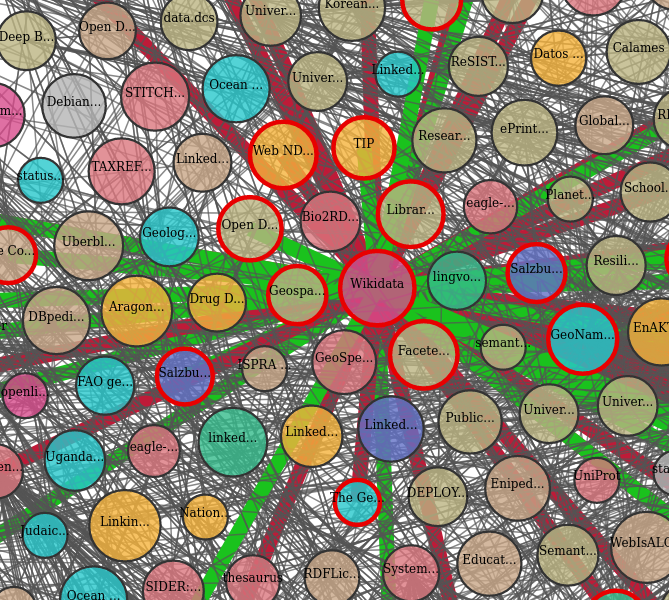
\includegraphics[width=0.625\textwidth]{lod_zoom.png}
            \captionof{figure}{Zoom de la \textit{Linked Open Data Cloud}}
            \label{fig:lod}
        \end{figure}
        
        \noindent En la \hyperref[fig:lod]{figura 1} se puede apreciar una pequeña parte de la \textit{Linked Open Data Cloud} \cite{LOD}, que refleja todos los conjuntos de datos abiertos y enlazados publicados, así como las relaciones entre los mismos. Esta inmensa ``nube" evidencia el poder y el valor de esta forma de publicación de datos, capaz de conformar una red de conocimiento muy amplia.
        \\ \\
        A diferencia de otros modelos de almacenamiento y gestión de la información, como las bases de datos convencionales, en los que se necesitan mecanismos auxiliares para reflejar esta referenciación e interconexión de datos, los datos enlazados poseen de manera intrínseca estas relaciones. Esta diferencia radica en la forma en la que se describen los datos: la web del hipertexto, la que estamos acostumbrados a explorar, suele estar descrita mediante el lenguaje \texttt{HTML} (por sus siglas en inglés, \textit{HyperText Markup Language} \cite{HTML}), mientras que la \textit{Web Semántica} se describe mediante el modelo \texttt{RDF} (\textit{Resource Description Framework}, en inglés \cite{RDF}).
        \\ \\
        
        \begin{figure}[h]
            \centering
            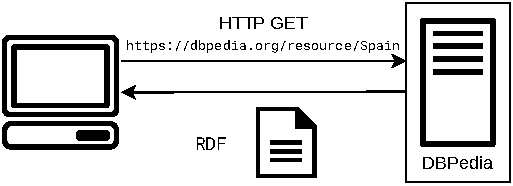
\includegraphics[]{linked.pdf}
            \captionof{figure}{Ejemplo de una consulta de datos enlazados}
            \label{fig:linked}
        \end{figure}

        \noindent A modo de ejemplo, y con el objetivo de reflejar algunos de los principios básicos de los datos enlazados, se muestra en la \hyperref[fig:linked]{figura 2} un caso de uso de una consulta sobre datos enlazados. La consulta es simple: un equipo solicita el recurso que representa la entidad de España al servidor de \textit{DBpedia} \cite{DBPEDIA}, uno de los proyectos más ambiciosos de la ``Web Semántica", que busca extraer la información de la más amplia enciclopedia \textit{online}, \textit{Wikipedia}, para generar datos enlazados.
        \\ \\
        En el ejemplo se pueden ver algunas de las peculiaridades de los datos enlazados:
        \begin{itemize}
            \item Uso de \texttt{URI}s como identificadores: con el objetivo de evitar ambigüedades y poder ofrecer una forma estandarizada y unívoca de identificación de entidades, todos los recursos se identifican mediante una \texttt{URI} (por su traducción del inglés, Identificador de recursos uniforme). Por lo tanto, una \texttt{URI} no es sólo una dirección, sino también un identificador: en el ejemplo, \texttt{\url{https://dbpedia.org/resource/Spain}} es la dirección en la que se aloja el recurso, pero también es el identificador que permite a cualquier otro sistema reutilizar dicho recurso.
            \item Protocolo \texttt{HTTP}: para evitar la multiplicidad de esquemas de \texttt{URI}s, se utiliza \texttt{HTTP} para asegurar que cualquier recurso pueda ser buscado y accedido en la Web.
            \item Obtención de recursos mediante \texttt{RDF}: Una vez se ha realizado una búsqueda y se pretende acceder a un recurso identificado por su \texttt{URI}, se obtiene una respuesta en forma de documento en formato \texttt{RDF}, que será explicado con más precisión en la \hyperref[subsubsec:RDF]{posterior sección}. Además, la forma de realizar consultas estructuradas sobre datos enlazados más allá de su obtención mediante \texttt{URI}s será descrita en \hyperref[subsubsec:SPARQL]{otra sección}.
        \end{itemize}
        
        \subsubsection{Modelo de datos \texttt{RDF}} \label{subsubsec:RDF}
            Si bien debido a la comparación previa entre la Web estándar y la denominada ``Web Semántica" podría parecer que \texttt{RDF} es un lenguaje de marcado de texto como lo es \texttt{HTML}, esto no es así: \texttt{RDF} es un \textit{framework} de representación de información: un modelo que permite codificar la información, sus propiedades, y las relaciones entre sí.
            \\ \\
            La sintaxis de este modelo es simple: se basa en conjuntos de tripletas de la forma sujeto-predicado-objeto, donde éstos pueden ser \texttt{URI}s, literales o elementos vacíos. Mediante estos conjuntos de definiciones se pueden construir \textit{datasets}, que a su vez se pueden organizar en grafos de conocimiento; estructuras con una alta riqueza en términos de información.
            \\ \\
            
            \begin{lstlisting}[language=lXML2,gobble=14]
                <http://dbpedia.org/resource/Spain>
                    <http://www.w3.org/1999/02/22-rdf-syntax-ns#type>	
                    <http://schema.org/Country> .
                <http://dbpedia.org/resource/Spain>
                    <http://dbpedia.org/ontology/currencyCode>
                    "EUR" .
                <http://dbpedia.org/resource/Spain>
                    <http://www.w3.org/2002/07/owl#sameAs>
                    <http://openei.org/resources/Spain> .
            \end{lstlisting}
            \captionof{figure}{Ejemplo de tripletas del modelo \texttt{RDF}}
            \label{fig:triplets}
            
            \vspace{0.7cm}
            
            En la \hyperref[fig:triplets]{figura 3} se pueden apreciar algunas de las tripletas que se otorgarían como respuesta a una petición como la de la \hyperref[fig:linked]{figura 2}. En \textcolor{Cerulean}{azul} aparecen los sujetos de las tripletas, mientras que en \textcolor{ForestGreen}{verde} y en \textcolor{BrickRed}{rojo} aparecen los predicados y los objetos, respectivamente.
            \\ \\
            La información de las tripletas, como se explicó previamente, está codificada mediante \texttt{URI}s, nodos vacíos o literales que representan entidades, propiedades y relaciones. En este caso, la primera tripleta nos dice que la entidad que representa a España es de tipo (\textcolor{ForestGreen}{\texttt{type}}) país (\textcolor{BrickRed}{\texttt{Country}}). La segunda, que en España el tipo de moneda (\textcolor{ForestGreen}{\texttt{currencyCode}}) tiene un código (\textcolor{BrickRed}{\texttt{EUR}}), que es un literal. La última de ellas establece una relación de identidad (\textcolor{ForestGreen}{\texttt{sameAs}}) entre el recurso \textcolor{Cerulean}{\texttt{http://dbpedia.org/resource/Spain}} y el recurso \textcolor{BrickRed}{\texttt{http://openei.org/resources/Spain}}, que se encuentran en distintos dominios.
            \\ \\
            En este ejemplo también pueden ser destacados otros elementos característicos de \texttt{RDF}: los vocabularios. Para expresar las propiedades (como \textcolor{ForestGreen}{\texttt{type}} o \textcolor{ForestGreen}{\texttt{sameAs}}), que potencialmente pueden aparecer en múltiples \textit{datasets}, es de interés poder contar con un índice de términos que poder reutilizar, siguiendo uno de los principios fundamentales de los datos abiertos y enlazados. Ésa es la función de proyectos como \textit{Linked Open Vocabularies} \cite{LOV}, que recoge a modo de códice todos los términos publicados como datos abiertos.
            \\ \\
            Un último apunte sobre \texttt{RDF} y el ejemplo provisto; como previamente se explicó sobre \texttt{RML}, éste no es un lenguaje de marcado sino un \textit{framework} que refleja cómo deben de ser los datos enlazados para que sigan los principios que los rigen. El ejemplo de la \hyperref[fig:linked]{figura 3} está codificado mediante el formato \texttt{N-Triples} \cite{NTRIPLES} (un subconjunto del formato \texttt{Turtle} \cite{TURTLE}). Sin embargo, existen otros formatos, como \texttt{JSON-LD} \cite{JSONLD}, \texttt{RDF/XML} \cite{RDFXML}, \texttt{RDFa} \cite{RDFA} o \texttt{N-Quads} \cite{NQUADS}.
        
        \subsubsection{Consultas sobre datos enlazados} \label{subsubsec:SPARQL}
            De la misma manera que para la realización de consultas sobre bases de datos convencionales se tiene el lenguaje \texttt{SQL} \cite{ISOSQL}, para construir búsquedas estructuradas sobre grafos de conocimiento de datos enlazados se utiliza \texttt{SPARQL} \cite{SPARQL}.
            \\ \\
            \texttt{SPARQL} trabaja con los datos en formato \texttt{RDF} y contiene las capacidades para la consulta de los patrones obligatorios y opcionales de grafo, junto con sus conjunciones y disyunciones. La sintaxis de \texttt{SPARQL} es similar a la de su análogo de bases de datos relacionales; en la \hyperref[fig:sqlsparql]{figura 4} se puede apreciar una consulta similar mediante los dos lenguajes:
            \\ \\
        
            \begin{figure}[h]
                \centering
                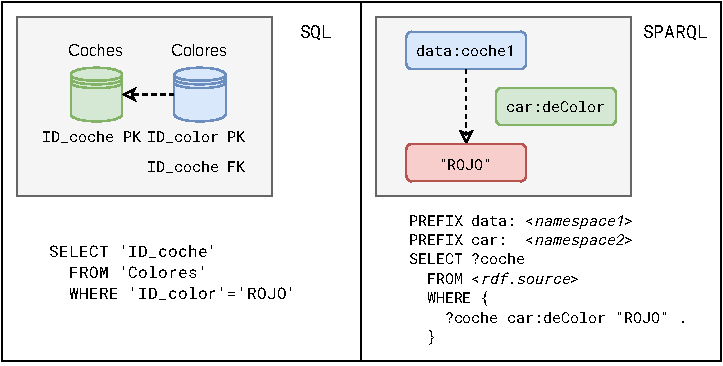
\includegraphics[]{sqlsparql.pdf}
                \captionof{figure}{Ejemplo de consultas en lenguajes \texttt{SQL} y \texttt{SPARQL}}
                \label{fig:sqlsparql}
            \end{figure}
            
            \noindent Las dos consultas muestran similitudes en distintos aspectos, como las cláusulas (\texttt{SELECT}, \texttt{FROM}, \texttt{WHERE}...) o la estructura de la sentencia, pero también evidencian las diferencias entre los lenguajes y los modelos tanto de bases de datos relacionales, como el modelo \texttt{RDF}: las consultas \texttt{SQL} se realizan sobre unos datos estructurados y sus atributos, teniendo que conocer por anticipado dicha estructura para poder construir la sentencia. En cambio, mediante \texttt{SPARQL} se pueden consultar directamente las tripletas del conjunto de datos. Además, este protocolo permite el uso de prefijos para ejecutar las consultas sobre elementos en dominios diversos.
            \\ \\
            Existen diversos sistemas que implementan, mediante \textit{API}s o \textit{triplestores} (un tipo de base de datos \textit{ad-hoc} para datos enlazados), sistemas con mecanismos de construcción de consultas \texttt{SPARQL}. Algunas de dichas implementaciones son:
            \\
            \begin{itemize}
                \item Apache Jena \cite{JENA}: \textit{framework} de código abierto escrito en el lenguaje \texttt{Java} para el desarrollo de aplicaciones sobre datos \texttt{RDF}.
                \item RDFLib \cite{RDFLIB}: biblioteca en \texttt{Python} para el procesado de datos en formato \texttt{RDF/XML} y sus grafos de conocimiento asociados. Utilizada  \hyperref[subsec:rdflib]{posteriormente} en el trabajo.
                \item RDF4J \cite{RDF4J}: previamente conocido como \textit{OpenRDF Sesame}, es otro \textit{framework} de código abierto escrito en el lenguaje \texttt{Java}.
                \item Virtuoso \cite{VIRTUOSO}: \textit{middleware} que combina las funcionalidades de un gestor de bases de datos relacionales convencionales con el procesado de datos enlazados.
            \end{itemize}
        
    \subsection{Licitaciones públicas}
        \subsubsection{Estándar \texttt{CODICE}}
            \texttt{CODICE} es una librería de componentes y documentos electrónicos \texttt{XML} estándar para el desarrollo de aplicaciones de contratación pública electrónica de conformidad con los procedimientos y prescripciones de las directivas \texttt{2014/23/UE} \cite{UE201423}; \texttt{2014/24/UE} \cite{UE201424}; \texttt{2014/25/UE} \cite{UE201425}; \texttt{2009/81/CE} \cite{UE200981} y de la normativa española en materia de contratación pública \cite{BOE20179}, así como con los estándares y recomendaciones internacionales aplicables a la identificación, denominación, definición y construcción de dichos componentes.
            \\ \\
            El proyecto \texttt{CODICE} persigue proporcionar a todo el Sector Público una arquitectura de componentes, documentos y mensajes \texttt{XML} estandarizados, conforme con las normas y estándares internacionales aplicables, que pueda ser usada por todos los sistemas, aplicaciones y componentes informáticos necesarios para la construcción de soluciones interoperables de contratación electrónica.
            \\ \\
            La finalidad del proyecto es asegurar la interoperabilidad, tanto de los subsistemas de contratación electrónica entre sí (Plataforma de Contratación Pública, registros electrónicos de empresas, catálogos electrónicos, sistemas de subastas electrónicas, etc.), como con los sistemas de información de los agentes económicos participantes en los procesos de contratación y con los de los propios órganos de las Administraciones Públicas.
            \\
        
            \begin{figure}[h]
                \centering
                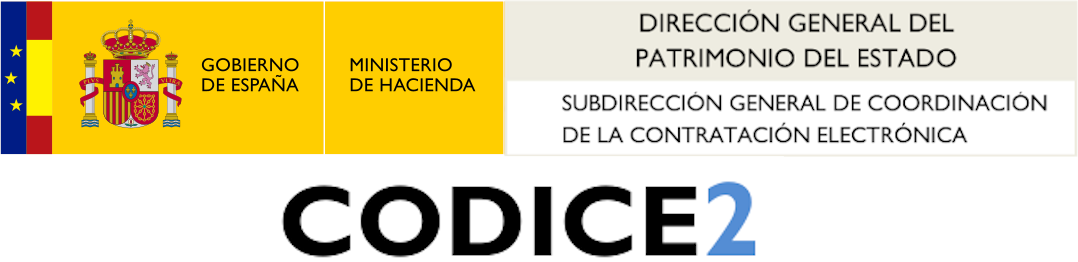
\includegraphics[width=\textwidth]{codice.png}
                \captionof{figure}{Logo del estándar \texttt{CODICE} (versión 2)}
            \end{figure}
            
            \noindent Para acomodar de forma armónica y coordinada las variadas necesidades y condicionantes de los distintos usuarios potenciales de los sistemas de contratación electrónica a desplegar, así como para facilitar la interoperabilidad de la plataforma de contratación pública y sus distintos subsistemas con las infraestructuras técnicas, organizativas y de información de todos los participantes en los procesos de contratación pública, se ha definido una arquitectura \cite{CODICEIMPL} que proporciona tanto los componentes comunes esenciales del sistema (definiciones y denominaciones normalizadas, componentes o módulos elementales reutilizables, documentos electrónicos de uso común, etc.), como la estructura y reglas que permite su extensión o adaptación a las necesidades especiales de diferentes contextos específicos de contratación.
            \\ \\
            Dicha arquitectura proporciona a los sistemas a desarrollar posteriormente los “bloques” o componentes básicos de información, así como las reglas de composición necesarias para la construcción de los documentos y mensajes electrónicos que licitadores y órganos de contratación han de intercambiarse a lo largo de los procesos de contratación, garantizando al mismo tiempo la interoperabilidad de todos los elementos cuya interacción proporcionará las funcionalidades necesarias para hacer efectiva la contratación electrónica \cite{CODICEFORM}.
            \\ \\
            Las normas y estándares internacionales existentes, tales como las normas ISO 11179 \cite{ISOMDR} y 15000 \cite{ISOEBXML}, los estándares ebXML de OASIS \cite{EBXML} y UN/CEFACT \cite{UNCEFACT}, y las Recomendaciones del W3C sobre lenguaje y esquema XML \cite{XML}, junto con las iniciativas promovidas por el programa IDA de la Unión Europea en relación con la contratación electrónica \cite{UEIDA}, han proporcionado la base para la definición y construcción de una arquitectura interoperable de información \cite{CODICE}.
            \\ \\
            En el portal institucional del Ministerio de Hacienda, concretamente en la sección de licitaciones publicadas en la Plataforma de Contratación del Sector Público \cite{PORTALHAC}, se pueden encontrar los documentos de licitaciones elaborados por la Dirección General del Patrimonio del Estado a partir de los datos que introducen los órganos de contratación como responsables de sus perfiles de contratantes. Estos documentos siguen el esquema \texttt{CODICE}, si bien no en todos los documentos van a aparecer los mismos elementos, dado que se proporcionan tres distintos tipos de documentos: licitaciones publicadas en la Plataforma de Contratación del Sector Público (excluyendo contratos menores), licitaciones publicadas mediante mecanismos de agregación y licitaciones correspondientes a contratos menores \cite{CODICETIPOS}. Este trabajo se ha centrado en el primero de los tipos previamente descritos, que incluye como superconjunto al tercero, el de los contratos menores.
            
        \subsubsection{Estándar \texttt{OCDS}}
            El Estándar de Datos para las Contrataciones Abiertas (\texttt{OCDS}, por sus siglas en inglés) permite la divulgación de datos y documentos de todas las etapas del proceso de contratación mediante la definición de un modelo de datos común. Se creó para apoyar a las organizaciones a aumentar la transparencia de la contratación y permitir un análisis más profundo de los datos de contrataciones por una amplia gama de usuarios \cite{OCDS}.
        
            \begin{figure}[h]
                \centering
                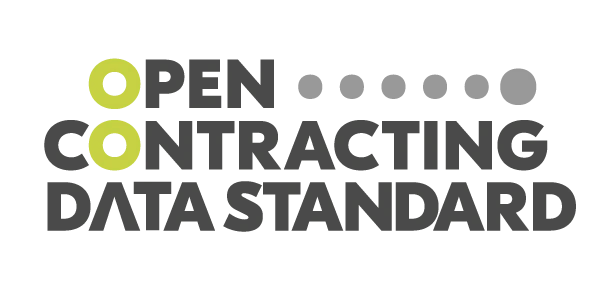
\includegraphics[width=0.625\textwidth]{ocds.png}
                \captionof{figure}{Logo del estándar \texttt{OCDS}}
            \end{figure}
            
            \noindent \texttt{OCDS} es un estándar de datos abierto, gratuito y no protegido por derechos de propiedad intelectual para la contratación pública, implementado por más de 30 gobiernos en todo el mundo. Es el único estándar abierto internacional para la publicación de información relacionada con la planeación, licitación e implementación de contratos públicos y ha sido avalado por el G20, el G7 e importantes organizaciones internacionales.
            \\ \\
            \texttt{OCDS} describe cómo publicar datos y documentos en todas las etapas del proceso de contratación. Fue creado para brindar apoyo a las organizaciones con el objetivo de aumentar la transparencia en las contrataciones y permitir un análisis más exhaustivo de los datos sobre contrataciones por parte de una amplia variedad de usuarios. \texttt{OCDS} brinda:
            
            \begin{itemize}
                \item Una serie de campos de datos y documentos para publicación recomendados
                \item Un modelo de datos estructurado común
                \item Orientación y herramientas para la implementación y el uso de datos
                \item Perfiles para asociaciones público-privadas, proyectos de infraestructura, la Unión Europea y el Acuerdo sobre Contratación Pública de la Organización Mundial del Comercio
                \item Un mecanismo de extensión para incorporar información adicional clave a sus datos de \texttt{OCDS}
                \item Un servicio de asistencia global gratuito
            \end{itemize}
            
            \noindent Los datos sobre contrataciones publicados en un formato de \texttt{OCDS} resultan más fáciles de compartir, comparar y analizar. Permiten que quienes los publican adapten y reutilicen las herramientas existentes de visualización y análisis como éstas \cite{OCDSTOOLS}, lo cual reduce los costes y favorece la innovación. \texttt{OCDS} ofrece orientación sobre qué publicar y cómo publicar los detalles más importantes sobre contratación pública identificados por profesionales, investigadores y otras partes interesadas.
            \\ \\
            \texttt{OCDS} fue concebido para atender cuatro necesidades específicas de los usuarios, en función de un análisis campo por campo de cómo pueden utilizarse los datos para dar respuesta a tales necesidades. Estas son:
            
            \begin{itemize}
                \item Lograr mayores beneficios a cambio del dinero que se paga, con lo cual se permite que el gobierno ahorre tiempo y dinero.
                \item Generar un entorno de negocios más justo y condiciones equitativas para los proveedores.
                \item Mejorar la integridad pública al desalentar el fraude y la corrupción.
                \item Hacer un seguimiento de la prestación de los servicios y mejorarlos.
            \end{itemize}
            
            Si se incorporan a reformas más amplias, los gobiernos pueden utilizar las contrataciones abiertas para obtener mayores beneficios a cambio del dinero que se paga por los bienes, las obras y los servicios y para ganarse la confianza del sector privado, la sociedad civil y la ciudadanía \cite{OCDSOC}.
            \\
            
            \begin{figure}[h]
                \centering
                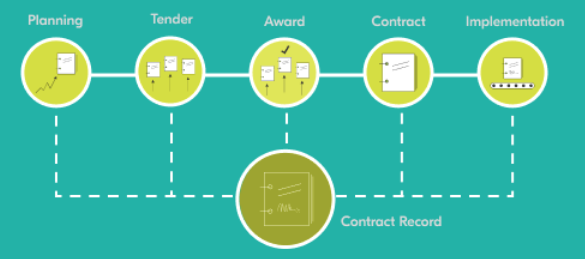
\includegraphics[width=0.67\textwidth]{tenderprocess.png}
                \captionof{figure}{Modelo del proceso de licitaciones en \texttt{OCDS}}
                \label{fig:tenderprocess}
            \end{figure}
            
            \noindent El proceso de licitaciones (véase \hyperref[fig:tenderprocess]{figura 7}), si bien sigue un modelo lineal, no siempre ha de cumplirse estrictamente de esa manera, dado que no todas las contrataciones pasan por todas las etapas, o en algunos casos es necesario proveer nueva información sobre una etapa previa.
            \\ \\
            Un documento \texttt{OCDS} está compuesto por bloques, íntegramente relacionados con el modelo del proceso de licitaciones \cite{OCDSBLOCKS}:
            
            \begin{itemize}
                \item \texttt{parties}: información sobre las organizaciones y otros participante involucrados en el proceso de contratación.
                \item \texttt{planning}: información sobre los objetivos, presupuestos y proyectos a los que se refiere un proceso de contratación.
                \item \texttt{tender}: información sobre la forma en que tendrá lugar la licitación o su realización.
                \item \texttt{awards}: información sobre las adjudicaciones otorgadas como parte de un proceso de contratación.
                \item \texttt{contracts}: información sobre contratos firmados como parte de un proceso de contratación.
                \begin{itemize}
                    \item \texttt{implementation}: información sobre el progreso de cada contrato hasta su finalización.
                \end{itemize}
            \end{itemize}
            
    \subsection{\textit{TheyBuyForYou}}
        \textit{TheyBuyForYou} (en adelante, \texttt{TBFY}) es un consorcio de empresas, universidades, centros de investigación, departamentos gubernamentales y autoridades locales de diversos países europeos, concretamente Reino Unido, Noruega, Italia, España y Eslovenia.
        \\ \\
        
        \begin{figure}[h]
            \centering
            
\includegraphics[width=0.5\textwidth]{tbfy.png}
            \captionof{figure}{Logo del proyecto \texttt{TBFY}}
        \end{figure}
        
        \noindent El proyecto de \texttt{TBFY} comenzó en enero de 2018 con el objetivo de mejorar el estado del mercado de adquisiciones europeo mediante el desarrollo de herramientas y funcionalidades que permitan explorar los datos abiertos en el ámbito de las licitaciones públicas. Para situarlo en contexto, ya hay diferentes organizaciones aprovechando el uso de las herramientas desarrolladas por el equipo de \texttt{TBFY}; el gobierno de Eslovenia las utiliza para identificar patrones que pudieran ser indicadores de fraude y autoridades españolas las usan para tomar decisiones de contrataciones más transparentes, entre otros casos.
        \\ \\
        El mercado de licitaciones europeo es tan grande que su navegación por parte de administraciones públicas, licitadores y empresas es complejas; es por ello que habitualmente grandes compañías consiguen contratos por encima de pequeños suministradores. \texttt{TBFY} quiere cambiar esto mediante la construcción de un gran grafo de conocimiento que recoja millones de datos sobre contrataciones públicas en el ámbito europeo. Siguiendo los principios que rigen los datos abiertos, los recursos de \texttt{TBFY} son públicos y de acceso abierto \cite{TBFY}.
        \\ \\
        
        \begin{figure}[h]
            \centering
            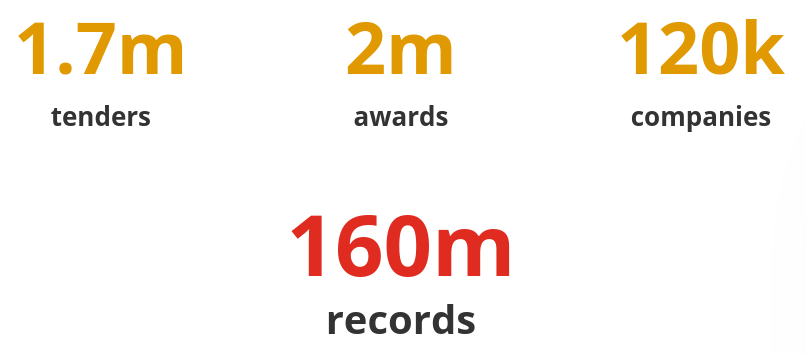
\includegraphics[width=0.625\textwidth]{tbfykg.png}
            \captionof{figure}{Dimensiones del grafo de conocimiento de \texttt{TBFY} (mayo de 2021)}
        \end{figure}
        
        \noindent Los datos recogidos en el grafo de conocimiento de \texttt{TBFY} son accesibles mediante \textit{endpoints} \texttt{SPARQL}, nodos sobre los cuales se pueden realizar peticiones mediante el protocolo \texttt{HTTP} y obtener respuestas en distintos formatos. Además, \texttt{TBFY} proporciona otras herramientas; el repositorio central \cite{TBFYREPOS}, una aplicación de búsquedas construida mediante \texttt{OptiqueVQS} (\textit{Visual Query System over Ontologies}) \cite{TBFYVQS}, una herramienta capaz de encontrar patrones anómalos en datos de contrataciones \cite{TBFYANOM}, etc.
        \\ \\
        Mediante el uso de la aplicación desarrollada en la \hyperref[sec:software]{posterior sección}, se generarán datos abiertos y enlazados capaces de ser explotados mediante algunas de las herramientas de \texttt{TBFY}.

\newpage